\section{Theorie}
\label{sec:Theorie}

\subsection{Allgemein}

Wenn äußere Kräfte auf einen Körper wirken, sodass 
sich dieser verformt, können Spannungen auftreten.
Dieses Verhalten kann der Abbildung \ref{fig:theorie1}
entnommen werden.

\begin{figure}[h]
    \centering
    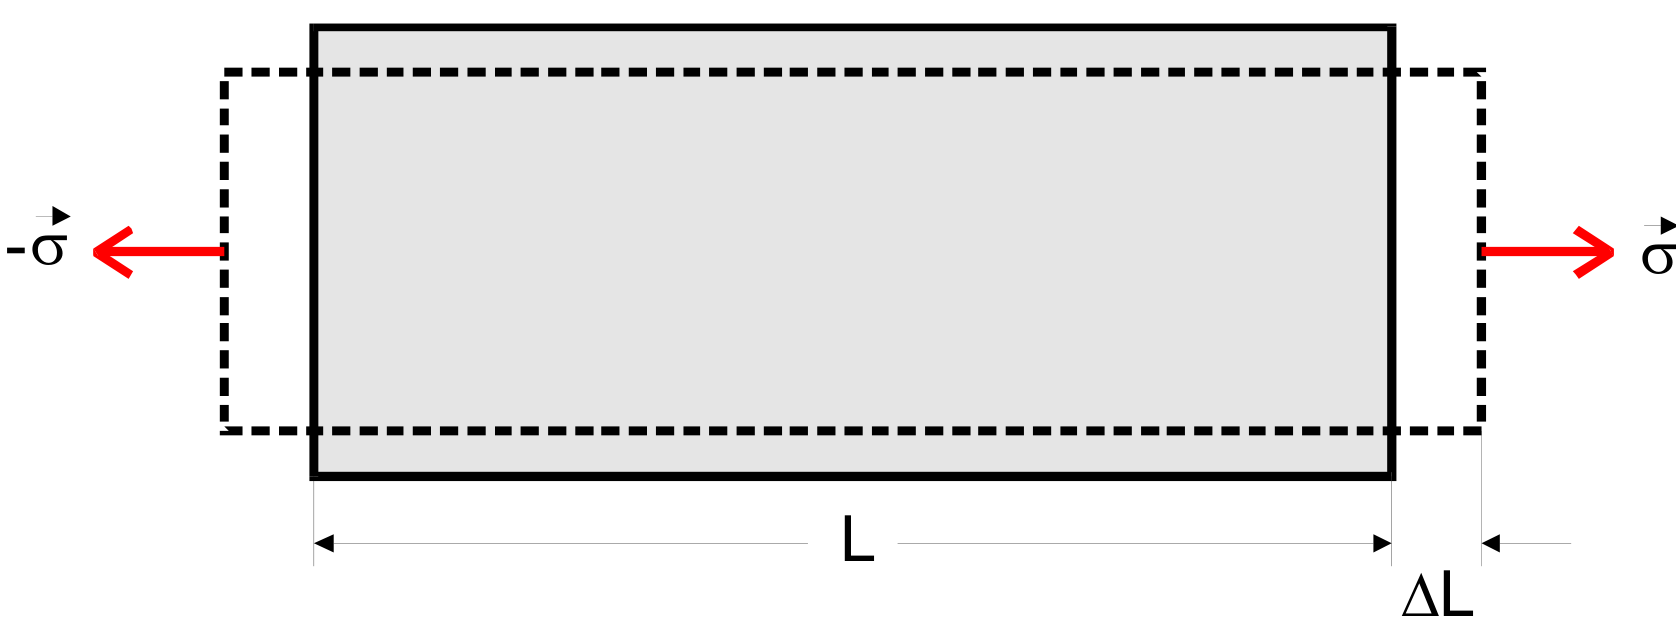
\includegraphics[width=10cm]{Theorie1.png}
    \label{fig:theorie1}
    \caption{Dehnung eines Stabes durch den Einfluss einer Normalspannung}
\end{figure}
\noindent
Es wird unterschieden zwischen der Normalspannung,
welche senkrecht zur Oberfläche steht und der 
Tangentialspannung, welche parallel zur Oberfläche 
verläuft. Wird durch eine von außenwirkende Kraft 
die Länge L eines Materials um $\Delta L $verkürzt, 
so entsteht eine Spannung, welche mithilfe
des Hookschen Gesetzes
\begin{equation}
    \sigma = E \frac{\Delta L}{L}
    \label{eq:1}
\end{equation}
\noindent beschrieben werden kann, wobei $E$ als
Elastizitätsmodul bezeichnet wird. Dieser 
Proportionalitätsfaktor lässt sich auch über die 
Biegung eines Stabes berechnen.


\subsection{Einseitige Biegung des Stabes}

Wird ein Stab, wobei die geometrische Form des 
Querschnitts allgemein nicht von Bedeutung für den
Ablauf des Versuchs ist, an einem seiner Enden
eingespannt und zusätzlich an dem anderen Ende mit 
einem Gewicht belastet, so lässt sich beobachten,
dass die Durchbiegung des Stabes mit zunehmenden
Abstand von dem eingespannten Ende ebenfalls 
zunimmt (siehe dazu Abbildung \ref{fig:theorie2}.

\begin{figure}[h]
    \centering
    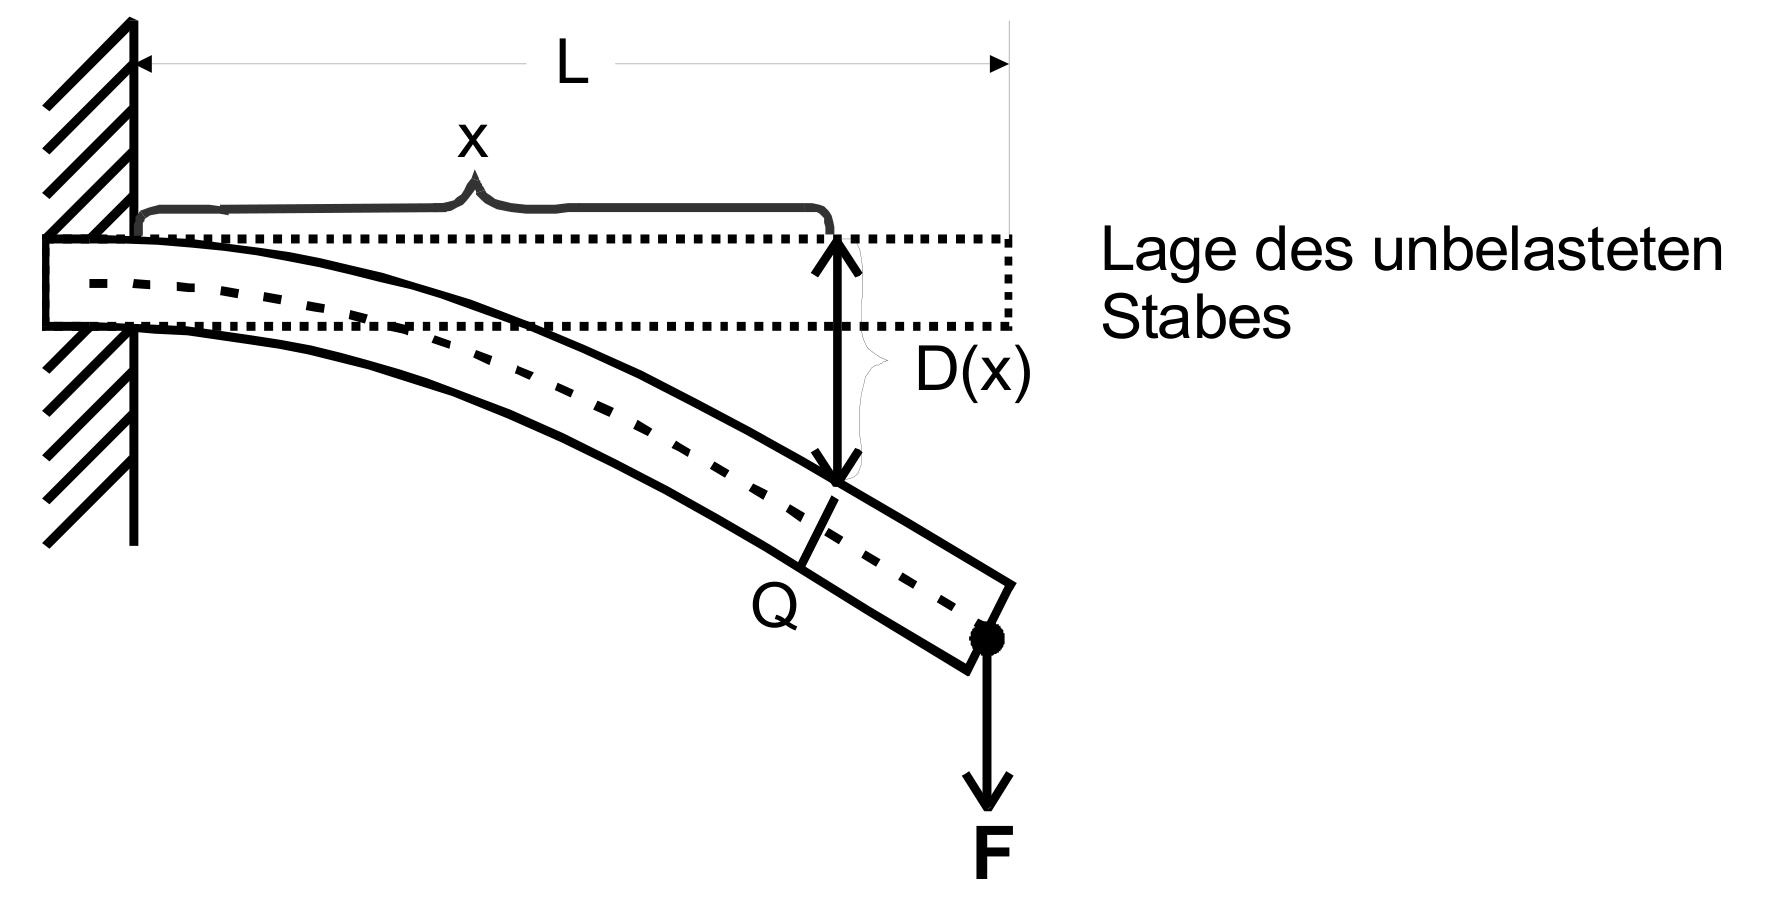
\includegraphics[width=10cm]{Theorie2.png}
    \label{fig:theorie2}
    \caption{Durchbiegung eines elastischen Stabes unter dem Einfluss einer Kraft bei einseitige Einspannung}
\end{figure}
\noindent
Durch die an der Stelle L wirkenden Kraft, wird auf
die an Querschnittsfläche an der Stelle x ein 
Drehmoment $M_F$ ausgeübt, welches eine Verdrehung 
des Stabes hervorruft. Die oberen Schichten des 
Stabes werden gestreckt und die unteren gestaucht. 
Der Stab verdreht sich so lange weiter, bis ein 
Gleichgewicht zwischen dem Drehmoment $M_F$
und dem durch die Spannungen zwischen den gestauchten
beziehungsweise gestreckten Schichten des Stabes 
enstehenden Drehmoments $M_{\sigma}$ entsteht.
Es existiert aber auch eine Schicht, in der keine 
Spannungen auftreten. Diese wird als neutrale
Faser bezeichnet.

Da die Kraft, die auf den Stab wirkt, senkrecht 
zu dem Kraftarm ist, gilt für das Drehmoment 
$M_F$, welches auf die Querschnittsfläche an der
Stelle $x$ wirkt
\begin{equation}
    M_F = F \cdot (L-x).
    \label{eq:2}
\end{equation}
\noindent
Im Gegensatz dazu lässt sich das Drehmoment 
$M_{\sigma}$ mit 
\begin{equation}
    M_{\sigma} = \int\limits_Q \! y \cdot \sigma (y) \, \mathrm{d}q
    \label{eq:3}
\end{equation}
\noindent berechnen, wobei y den Abstand des 
Flächenelements $dq$ von der neutralen Faser
angibt (siehe Abbildung \ref{fig:theorie 3}). 


\begin{figure}[h]
    \centering
    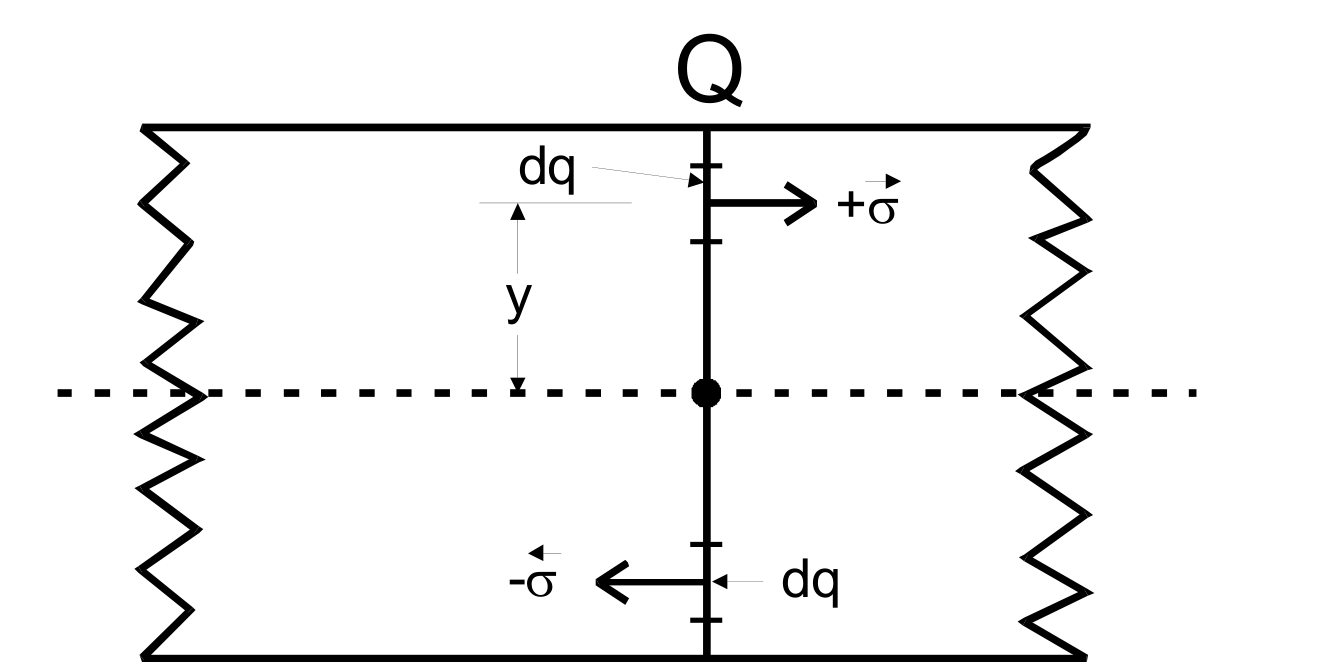
\includegraphics[width=10cm]{Theorie3.png}
    \label{fig:theorie1}
    \caption{Querrschnitt des Stabes zur Berechnung des Drehmoments $M_{\sigma}$}
\end{figure}
\noindent

Weiterhin kann $\sigma (y)$
mithilfe von Gleichung \ref{eq:1} umgeschrieben werden,
sodass sich 
\begin{equation}
    \sigma (y) = E \, \frac{\delta x}{\Delta x}
    \label{eq:4}
\end{equation}
\noindent ergibt. Hierbei gibt $\delta x$ die 
Änderung der Länge von $\Delta x$ infolge der
Biegung des Stabes.
 

\begin{figure}[h]
    \centering
    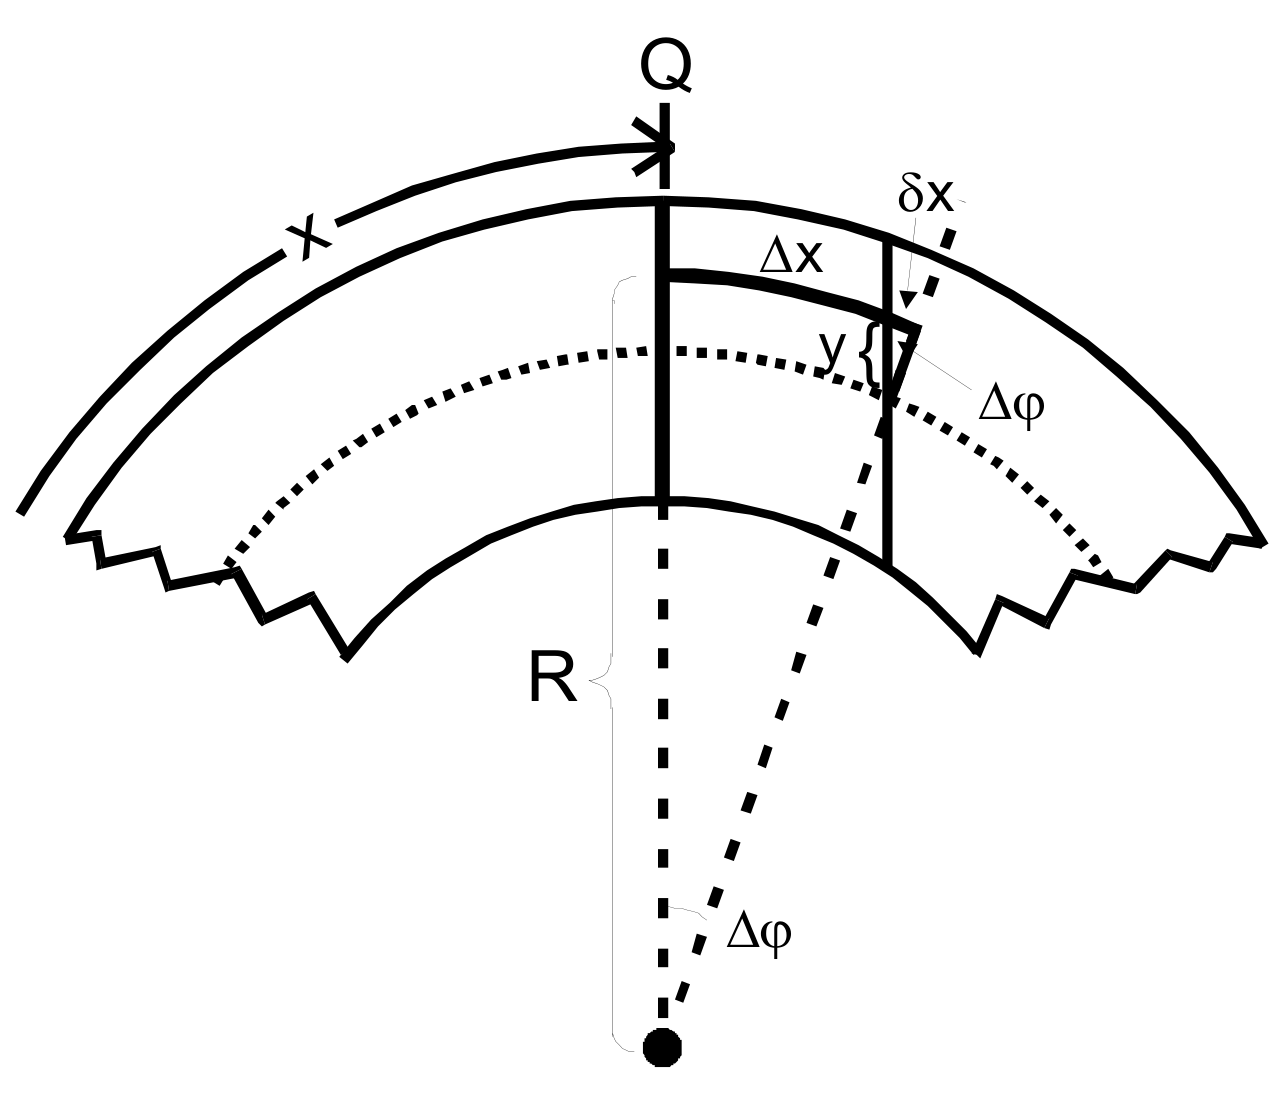
\includegraphics[width=10cm]{Theorie4.png}
    \label{fig:theorie4}
    \caption{Skizze zur Berechnung der Normalspannung $\sigma (y)$ in einem gebogenen Stab}
\end{figure}

\noindent
Aus der Abbildung \ref{fig:theorie4} lässt sich für 
$\delta x \ll \Delta x$ entnehmen, dass sich 
die Längenänderung $\delta x$ als 
\begin{equation}
    \delta x = y \Delta \phi = y \frac{\Delta x}{R}
    \label{eq:5}
\end{equation}
\noindent schreiben lässt. Mit der Annahme, dass mit 
$R$ ein geringer Krümmungsradius vorliegt, lässt sich
das Gleichgewicht von $M_F$ und $M_{\sigma}$ mit den
Gleichungen \ref{eq:2} und \ref{eq:3} zu 
\begin{equation}
    E\, \frac{\mathrm{d}^2 D}{\mathrm{d} x^2} \int\limits_Q \! y^2\, \mathrm{d}q = F(L-x)
    \label{eq:6}
\end{equation}
\noindent umformulieren. Das Integral
\begin{equation}
    I = \int\limits_Q \! y^2\, \mathrm{d}q
    \label{eq:7}
\end{equation}
\noindent wird als Flächenträgheitsmoment bezeichnet.
Zusammenfassend ergibt sich also für die gesuchte 
Durchbiegung $D(x)$ der Zusammenhang
\begin{equation}
    D(x) = \frac{F}{2 E I} \left( L x^2 - \frac{x^3}{3} \right)
    \label{eq:8}
\end{equation}
\noindent für $0 \leq x \leq L$.




\subsection{Zweiseitige Biegung eines Stabes}


\begin{figure}[h]
    \centering
    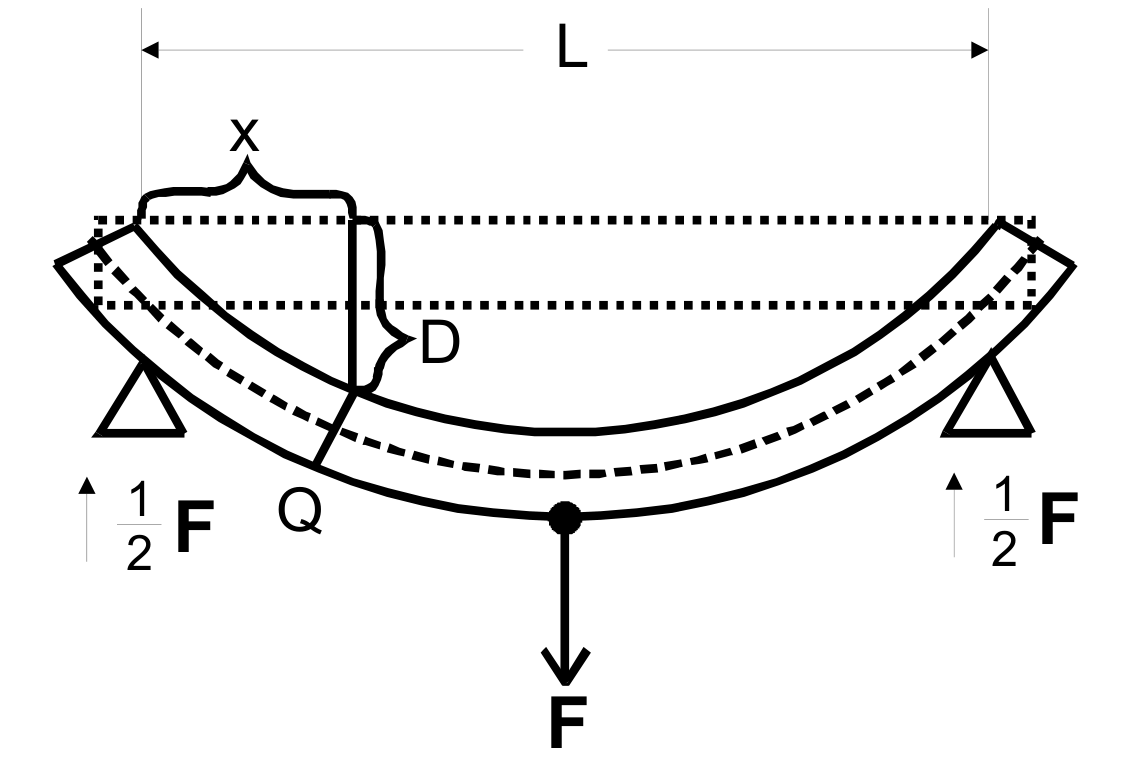
\includegraphics[width=10cm]{Theorie5.png}
    \label{fig:theorie5}
    \caption{Durchbiegung eines zweiseitig aufgelegten Stabes}
\end{figure}    
\noindent
Wenn ein Stab nun nicht nur an einem Ende, sondern
an seinen beiden Enden eingespannt wird, wie in 
der Abbildung \ref{fig:theorie5} zu sehen ist, greift nur 
noch das Drehmoment 
\begin{equation}
    M_{F} = -\frac{F}{2}x
    \label{eq:9}
\end{equation}
\noindent an der Querschnittsfläche Q an, für die
$0 \leq x \leq L/2$ gilt. Im Gegensatz dazu gilt für 
$L/2 \leq x \leq L$ nun 
\begin{equation}
    M_{F} = -\frac{F}{2}(L-x).
    \label{eq:10}
\end{equation}
Mittels dieser Gleichungen und der Annahme, dass 
in der Mitte des Stabes die Biegekurve $D(x)$ eine
horizontale Tangente besitzt, ergibt sich aus der Gleichung
\ref{eq:6}
für $0 \leq x \leq L/2$
\begin{equation}
    D(x) = \frac{F}{48 E I} \left( 3 L^2 x - 4 x^3 \right)
    \label{eq:11}
\end{equation}
\noindent beziehungsweise für $L/2 \leq x \leq L$
\begin{equation}
    D(x) = \frac{F}{48 E I} \left( 4 x^3 - 12 L x^2 + 9 L^2 x - L^3 \right).
    \label{eq:12}
\end{equation}
